%----------------------------------------------------------------------------
\documentclass[twocolumn,a4paper,11pt]{article}
\usepackage{times}
\usepackage{graphicx}
\usepackage{color}

\definecolor{Blue}{rgb}{0.4,0.4,0.9}

%----------------------------------------------------------------------------
\input{../../../util/tex/products}
\def\version{3.1}


%----------------------------------------------------------------------------
\def\cp{Constraint Programming}

%----------------------------------------------------------------------------
\begin{document}
\pagestyle{empty}
\onecolumn
\begin{center}
\ \\
\vspace{3cm} 
\makebox{
\includegraphics[width=13cm]{logo}}
\ \\
\vspace{3cm} 
{\huge \bf An overview of\\ {\jcs}}
\ \\
\vspace{.5cm}
Copyright 2002-2006 \koalog
\ \\
\vspace{4cm}
\begin{minipage}{9cm}
\begin{small}
{\sunlegal}
{\ibmlegal}
{\mslegal}
{\linuxlegal}
\end{small}
\end{minipage}
\end{center}

\newpage
\twocolumn
%----------------------------------------------------------------------------
\section*{\color{Blue}Introduction} 
{\jcs} is a {\java} library for solving combinatorial optimization problems 
using Constraint Programming or Local Search.

It provides cutting-edge technology for solving satisfaction and optimization problems, including:
\begin{itemize}
\item scheduling: {\jcs} provides a specific API for disjunctive scheduling;
\item resource allocation;
\item planning;
\item time tabling;
\item configuration: {\jcf} is powered by {\jcs};
\item and more generally, any type of satisfaction or optimization problem. 
\end{itemize}
{\jcs} includes solvers over integer, boolean and set domains, and a large
collection of predefined constraints.

{\jcs} allows ANYTIME constraint solving. 
It also includes a local search solver, useful for solving huge problems
where exact methods are too slow.

%----------------------------------------------------------------------------
\section*{\color{Blue}Available constraints}
{\jcs} comes with a large collection of constraints, in the following categories:
\begin{itemize}
\item arithmetic constraints (including sum, product, comparison, absolute value);
\item boolean constraints (including conjunction, disjunction, negation);
\item meta-constraints (including tests of relations such as equality, comparison);
\item global constraints (including alldifferent, colored matrix, cumulative, cycle,
  disjunctive, global cardinality constraint, latin square, permutation, sort).
\end{itemize}
Each of these constraints, in particular global constraints, 
contains state-of-the-art filtering algorithms.

%----------------------------------------------------------------------------
\section*{\color{Blue}Ease of use}
Usually, in {\cp}, 
the steps involved in the resolution of a problem are: 
\begin{itemize}
\item the modelling of the problem;
\item the design of a problem-specific solver or strategy.
\end{itemize}
{\jcs} {\java} API has been carefully designed such that its users
are not required to be constraint programming specialists or {\java} experts:
\begin{itemize}
\item the modelling of a problem is done through {\jcs} intuitively-named core classes;
\item {\jcs} core solvers are powerful and flexible enough to handle most problems,
eliminating the need in most cases to design a custom solver.
\end{itemize}

%----------------------------------------------------------------------------
\section*{\color{Blue}Open architecture}

{\jcs} is also a very open and extensible framework (figure \ref{fig:archi}
details the architecture of {\jcs}), 
with which advanced users can easily plug in extensions. 
\begin{figure}[htb]
\begin{center}
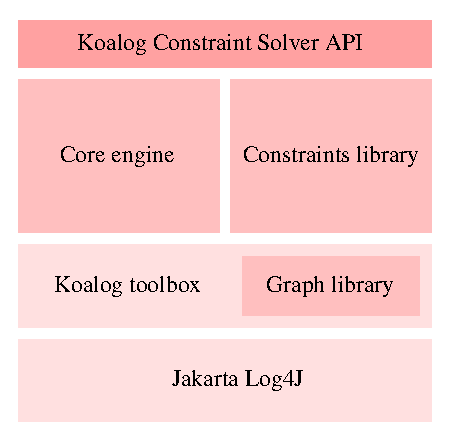
\includegraphics[width=7.5cm]{../archi}
\caption{\label{fig:archi}{\jcs} architecture}
\end{center}
\end{figure}
See table \ref{tab:extensions} for
examples of possible extensions of {\jcs}.
\begin{table}[htb]
\begin{center}
\begin{tabular}{|p{3cm}|p{4cm}|}
\hline
{\bf Extension}                                                 & {\bf Time
  required} (depending on the programmer skills and on the extension complexity)\\
\hline
\hline
Adding a new constraint                                         & from a couple of hours to a couple of days\\
\hline
Developing a new search strategy                                & from a couple of hours to a couple of days\\
\hline
Developing a new solver (soft solver, etc)                      & from a couple of days to a couple of weeks\\
\hline
\end{tabular}
\caption{\label{tab:extensions}Examples of {\jcs} possible extensions}
\end{center}
\end{table}



%----------------------------------------------------------------------------
\section*{\color{Blue}Quality}
{\jcs} has been produced to the highest quality standards:
\begin{itemize}
\item it is fully documented (Javadoc and tutorial);
\item it is fully internationalizable;
\item it is fully tested 
(it relies on {\junit}\footnote{{\junit} is an open source project initiated by Kent Beck (the author of ``Extreme Programming'').} 
and the {\koalog} Code Coverage utility for the tests);
\item it comes with a fully customizable logging system ({\log4j}\footnote{{\log4j} is an open-source project of the {\asf}.}).
\end{itemize}

%----------------------------------------------------------------------------
\section*{\color{Blue}Applications}
\subsubsection*{Commercial applications}
{\jcs} is currently used in an industry-level car configurator ({\jcf}) and in
various kinds of rota generators.

\subsubsection*{Research applications}
Code examples, showing how to solve classical problems such as 
\begin{itemize}
\item the Golomb ruler problem,
\item the travelling salesman problem,
\item the job-shop scheduling problem,
\item sport scheduling problems (including round-robin tournaments),
\item the car sequencing problem,
\item the partition problem,
\item the knapsack problem,
\item and many others
\end{itemize}
can be found on {\jcs} website:\\
{\tt http://www.koalog.com/php/jcs.php}.

%----------------------------------------------------------------------------
\section*{\color{Blue}Supported platforms}
{\jcs} is a {\java} library and thus smoothly integrates to any
{\java} application. See table \ref{tab:ports} for detailed information.

\begin{table}[htb]
\begin{center}
\begin{tabular}{|p{2.8cm}|c|c|c|c|}
\hline
                  & \multicolumn{4}{|c|}{{\java} Virtual Machine} \\ \cline{2-5}
Operating System  & \multicolumn{2}{|c|}{{\sun} {\jsdk}} & \multicolumn{2}{|c|}{{\ibm} JDK} \\ \cline{2-5}
                  & 1.4.2 & 1.5.0 & 1.4.2 & 1.5.0 \\
\hline
\hline
{\suse} 9.3           & yes & yes & yes & yes \\
{\fedoracore} 3       & yes & yes & yes & yes \\
{\windowsXP}          & yes & yes & n/a & n/a \\ 
{\solaris} Sparc 2.8  & yes & yes & n/a & n/a \\
\hline
\end{tabular}
\caption{\label{tab:ports}{\jcs} supported platforms}
\end{center}
\end{table}

%----------------------------------------------------------------------------
\section*{\color{Blue}Commercial information}
To evaluate or purchase the latest release of {\jcs} (v\version), 
please contact {\tt sales@koalog.com}.

%----------------------------------------------------------------------------
\end{document}

